%%
%% Automatically generated file from DocOnce source
%% (https://github.com/hplgit/doconce/)
%%
%%
% #ifdef PTEX2TEX_EXPLANATION
%%
%% The file follows the ptex2tex extended LaTeX format, see
%% ptex2tex: http://code.google.com/p/ptex2tex/
%%
%% Run
%%      ptex2tex myfile
%% or
%%      doconce ptex2tex myfile
%%
%% to turn myfile.p.tex into an ordinary LaTeX file myfile.tex.
%% (The ptex2tex program: http://code.google.com/p/ptex2tex)
%% Many preprocess options can be added to ptex2tex or doconce ptex2tex
%%
%%      ptex2tex -DMINTED myfile
%%      doconce ptex2tex myfile envir=minted
%%
%% ptex2tex will typeset code environments according to a global or local
%% .ptex2tex.cfg configure file. doconce ptex2tex will typeset code
%% according to options on the command line (just type doconce ptex2tex to
%% see examples). If doconce ptex2tex has envir=minted, it enables the
%% minted style without needing -DMINTED.
% #endif

% #define PREAMBLE

% #ifdef PREAMBLE
%-------------------- begin preamble ----------------------

\documentclass[%
oneside,                 % oneside: electronic viewing, twoside: printing
final,                   % draft: marks overfull hboxes, figures with paths
10pt]{article}

\listfiles               %  print all files needed to compile this document

\usepackage{relsize,makeidx,color,setspace,amsmath,amsfonts,amssymb}
\usepackage[table]{xcolor}
\usepackage{bm,ltablex,microtype}

\usepackage[pdftex]{graphicx}

\usepackage[T1]{fontenc}
%\usepackage[latin1]{inputenc}
\usepackage{ucs}
\usepackage[utf8x]{inputenc}

\usepackage{lmodern}         % Latin Modern fonts derived from Computer Modern

% Hyperlinks in PDF:
\definecolor{linkcolor}{rgb}{0,0,0.4}
\usepackage{hyperref}
\hypersetup{
    breaklinks=true,
    colorlinks=true,
    linkcolor=linkcolor,
    urlcolor=linkcolor,
    citecolor=black,
    filecolor=black,
    %filecolor=blue,
    pdfmenubar=true,
    pdftoolbar=true,
    bookmarksdepth=3   % Uncomment (and tweak) for PDF bookmarks with more levels than the TOC
    }
%\hyperbaseurl{}   % hyperlinks are relative to this root

\setcounter{tocdepth}{2}  % levels in table of contents

% Tricks for having figures close to where they are defined:
% 1. define less restrictive rules for where to put figures
\setcounter{topnumber}{2}
\setcounter{bottomnumber}{2}
\setcounter{totalnumber}{4}
\renewcommand{\topfraction}{0.95}
\renewcommand{\bottomfraction}{0.95}
\renewcommand{\textfraction}{0}
\renewcommand{\floatpagefraction}{0.75}
% floatpagefraction must always be less than topfraction!
% 2. ensure all figures are flushed before next section
\usepackage[section]{placeins}
% 3. enable begin{figure}[H] (often leads to ugly pagebreaks)
%\usepackage{float}\restylefloat{figure}

% prevent orhpans and widows
\clubpenalty = 10000
\widowpenalty = 10000

% --- end of standard preamble for documents ---


% insert custom LaTeX commands...

\raggedbottom
\makeindex
\usepackage[totoc]{idxlayout}   % for index in the toc
\usepackage[nottoc]{tocbibind}  % for references/bibliography in the toc

%-------------------- end preamble ----------------------

\begin{document}

% matching end for #ifdef PREAMBLE
% #endif

\newcommand{\exercisesection}[1]{\subsection*{#1}}


% ------------------- main content ----------------------



% ----------------- title -------------------------

\thispagestyle{empty}

\begin{center}
{\LARGE\bf
\begin{spacing}{1.25}
Quadrupole ion trap
\end{spacing}
}
\end{center}

% ----------------- author(s) -------------------------

\begin{center}
{\bf Bror Hjemgaard, René Ask og Sigurd Sørlie Rustad${}^{}$} \\ [0mm]
\end{center}

\begin{center}
% List of all institutions:
\end{center}
    
% ----------------- end author(s) -------------------------

% --- begin date ---
\begin{center}
Jul 26, 2020
\end{center}
% --- end date ---

\vspace{1cm}


\emph{In week-exercise (insert week exercise) we studied the Paul trap. Using both theoretical and numerical approximations we managed to trap ionized particles. Although the method worked in in theory, it is no guaranty it will work in practice. That is why, in this exercise we are going to apply the theory and try to build a working Paul trap.}

\section{Equipment list}
\label{title:equip_list}
Make sure you have all the equipment needed to do the experiment.
\begin{itemize}
  \item Transformer (one of the coils doubles as a voltage source, make sure it is NOT plugged in before the teaching assistant have approved your circuit!)

  \item Green laser pointer

  \item Two $1\rm{M}\Omega$ resistors

  \item Pinch cables

  \item One support stand

  \item Electrical tape

  \item Cinnamon (this is what we are going to use as ionized particles)

  \item Q-tips

  \item 3D printed trap
\end{itemize}

\noindent
\section{Building the trap}
\label{title:build}
First of all we need to set up the circuit. See figure~\ref{fig:circuit} and set up the circuit you see in the figure. Before plugging anything into the outlet, contact the teaching assistant to make sure everything is correctly set up.


\begin{figure}[!ht]  % fig:circuit
  \centerline{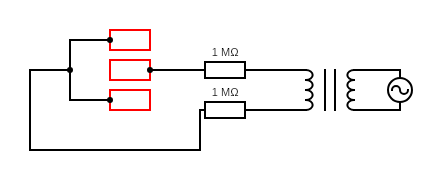
\includegraphics[width=0.9\linewidth]{figurer/circuit.png}}
  \caption{
  The figure shows the circuit of the setup. The red squares are the poles that will be charged during the experiment. \label{fig:circuit}
  }
\end{figure}
%\clearpage % flush figures fig:circuit


In order to better visualize the particles we are going to use the green laser pointer. Use the support stand and point the laser through the center of the ring in the trap.

\section{Experimenting}
\label{title:exp}
Now that the circuit is correctly set up, we can try to trap some particles. Turn off any light and plug the voltage source into a power outlet. Flip the switch of the voltage source to turn it on, and use a q-tip to feed some cinnamon inside the trap. Do you see trapped particles?

% ------------------- end of main content ---------------

% #ifdef PREAMBLE
\end{document}
% #endif

